i\section{Visione generale della strategia di verifica}
\sectionmark{Visione generale \dots}

La strategia generale adottata è quella di automatizzare il più possibile il lavoro di verifica; questo richiede scelta e uso di \glossario{tools} adeguatamente configurati. L'obiettivo è avere un riscontro affidabile e numericamente trattabile che permetta di assicurare il grado di qualità predeterminato. Il lavoro manuale verrà così ridotto al minimo e confinato all'opera di validazione.
La speranza è che dei buoni processi portino ad un buon software.
	
	\subsection{Organizzazione}
	Viene verificata la qualità di ogni processo e di ogni output da esso prodotto. Ogni fase  descritta nel \PianoDiProgetto{} produce output di diverso tipo, per questo è necessario programmare l'attività di verifica in modo mirato:

	\begin{itemize}
		\item \textbf{Analisi}: in questa fase si controllano che i processi e la documentazione prodotta rispettino le \emph{Norme di Progetto};
		\item \textbf{Progettazione Architetturale}: in questa fase vanno verificati i processi incrementali relativi all'analisi e ai nuovi documenti di progettazione;
		\item \textbf{Progettazione di Dettaglio e Codifica}: in questa fase vanno verificati i processi incrementali relativi alla progettazione.
	\end{itemize}
	
	Il \emph{Diario delle modifiche} viene incluso in ogni documento al fine di tracciarne uno storico dell'evoluzione.
	
	\subsection{Pianificazione strategica e temporale}
		\subsubsection{Strategia}

		Il \emph{Piano di Progetto} fissa una serie di scadenze improrogabili, pertanto è necessario definire con chiarezza una strategia di qualifica efficace. Gli incrementi sulla documentazione o sul codice possono essere di natura programmata, quindi prefissati nel calendario, oppure posso insorgere come inaspettati, in questo caso sarà necessario programmare le dovute modifiche; è questo il caso di \glossario{bug} o \emph{errori} (vedi paragrafo \ref{DefinizioneAnomalie}). La qualità di ogni incremento si basa sul fatto che la struttura di qualifica garantisce il rispetto delle \emph{Norme di Progetto}. Questo lavoro verrà svolto con l'aiuto di automatismi che segnaleranno le problematiche rilevate in modo da permettere una rapida correzione, in particolare:
		\begin{itemize}
			\item Documentazione: tramite uno script di \glossario{pre-commit} viene bloccato il commit nel \glossario{repository} se le modifiche eseguite impediscono la compilazione dei documenti o se gli strumenti di verifica automatica rilevano delle anomalie. In questo modo viene sempre garantita una qualità minima per il codice caricato sul \glossario{repository}.
			%\item Software: da definire.
		\end{itemize}

	Per migliorare l'efficienza dei processi si utilizzano quanto più possibile automatismi, in modo da poter destinare le risorse umane ad altri lavori. L'utilizzo di software apposito permette di eseguire controlli mirati senza consumare risorse umane. L'implementazione di tali controlli viene descritta nelle \NormeDiProgetto.
	
		\subsubsection{Tempistiche}
		La pianificazione strategica si basa sul modello \glossario{SEMAT}. Le seguenti specifiche non coprono tutti gli stati indicati da questo schema considerando solo l'aspetto relativo alla \textbf{qualità}. 
		
		Le sezioni coinvolte sono:
			\begin{itemize}
				\item \emph{Solution $\rightarrow$ Software System}: qualità del software;
				\item \emph{Endeavor $\rightarrow$ Way of Working}: qualità del ambiente di lavoro garantita dalle norme;
				\item \emph{Endeavor $\rightarrow$ Work}: qualità dei processi.
			\end{itemize}
		
	In questo modello viene fatta una distinzione tra lavoro e modo di lavorare, la qualità però è trasversale a queste due entità, per cui andrebbero considerati  anche alcuni aspetti della sezione \emph{work}. Per chiarezza è stato scelto di considerare il \emph{Way of Working} perché, in accordo con lo schema fornito da \glossario{SEMAT}, guida il lavoro stesso determinando la qualità prodotta.
		
	\begin{figure}[h]
	\centering 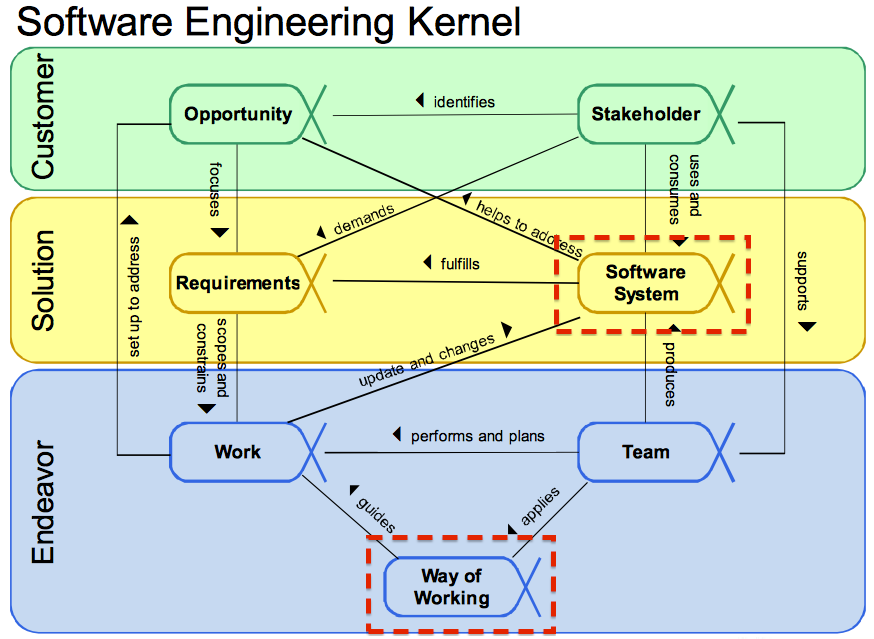
\includegraphics[width=1\textwidth]{Semat.png}
	\caption{Software Engineering Kernel}
	\end{figure}
	Di seguito viene descritto lo stato che ogni fase descritta dal \emph{Piano di Progetto} deve soddisfare, in relazione alle sezioni del \glossario{SEMAT} sopracitate.
   
   	\paragraph{Analisi}
    	\begin{itemize}
    		\item Software System:
    			\begin{enumerate}
    				\item \emph{Architecture Selected}: le piattaforme, le tecnologie e i linguaggi da usare sono stati selezionati. Vengono individuate le metriche per il software, i documenti ed i processi.
    			\end{enumerate}
    		\item Way of Working:
    			\begin{enumerate}
    				\item \emph{Principles Established}: i vincoli sono stati definiti nelle \NormeDiProgetto, i \glossario{tools} sono stati individuati ed il team comincia ad operare secondo quanto stabilito;
    				\item \emph{Foundation Established}: i \glossario{tools} per la qualità sono configurati e le buone pratiche da seguire sono definite;
    				\item \emph{In Use}: alcuni membri del team utilizzano le pratiche indicate e i tools vengono usati e migliorati. Vengono raccolti feedback sull'utilizzo degli strumenti per la qualità.
    			\end{enumerate}
    	\end{itemize}
    	
	\paragraph{Progettazione Architetturale}	
		\begin{itemize}
    		\item Software System:
    			\begin{enumerate}
    			\setcounter{enumi}{1}
    				\item \emph{Demonstrable}: le caratteristiche chiave dell'architettura software sono state individuate e gli \glossario{stakeholders} sono in accordo. Vengono individuate le unità da testare per soddisfare la richiesta del \glossario{proponente} di verificare il funzionamento di almeno il 70\% del software prodotto.
    			\end{enumerate}
    		\item Way of Working:
    			\begin{enumerate}
    			\setcounter{enumi}{3}
    				\item \emph{In Place}: tutti i membri utilizzano e comprendono l'intero ambiente di lavoro che è configurato secondo le \NormeDiProgetto. Il \glossario{repository} è configurato per accettare solo materiale in linea con le norme stabilite;
    				\item \emph{Working Well}: tutto il team lavora in modo coordinato secondo le norme applicando le pratiche individuate nelle 	norme e i \glossario{tools} supportano a pieno regime l'attività di lavoro.
    			\end{enumerate}
    			
    	\end{itemize}
    	
	\paragraph{Progettazione di Dettaglio e Codifica}	
		\begin{itemize}
    		\item Software System:
    			\begin{enumerate}
    			\setcounter{enumi}{2}
    				\item \emph{Usable}: il sistema è parzialmente usabile. Vengono praticati gli opportuni test che saranno convalidati ed il livello di anomalie sarà accettabile;
    				\item\emph{Ready}: la documentazione utente è disponibile ed è conforme alle norme. Vengono forniti i risultati dell'analisi statica e dei test eseguiti, si correggono le anomalie e gli \glossario{stakeholders} accettano il sistema.
    			\end{enumerate}
    	\end{itemize}
    	
	\paragraph{Verifica e Validazione}	
		\begin{itemize}
    		\item Software System:
    			\begin{enumerate}
    			\setcounter{enumi}{4}
    				\item \emph{Operational}: il sistema è in uso in un ambiente pienamente funzionante. Vengono ultimati gli ultimi test;
    				\item \emph{Retired}: il ritiro del software non viene considerato all'interno di questo progetto didattico.
    			\end{enumerate}
    		\item Way of Working:
    			\begin{enumerate}
    			\setcounter{enumi}{5}
    				\item \emph{Retired}: il ritiro del software non viene considerato all'interno di questo progetto didattico.
    			\end{enumerate}
    	\end{itemize}
	
		
	\subsection{Responsabilità}

	La responsabilità della verifica viene attribuita al \emph{Responsabile} di progetto e ai \emph{Verificatori}. I compiti e le modalità di attuazione sono definiti nel \emph{Piano di Progetto}.
	
	\subsection{Risorse}

	La qualifica dei processi essendo un processo, consuma delle risorse che si dividono in due categorie:
		\begin{itemize}
  			\item \textbf{Umane}: le figure coinvolte sono il \emph{Responsabile} di progetto e il \emph{Verificatore}. I processi da loro effettuati consumano ore di produttività contabilizzate e schedulate secondo il \emph{Piano di Progetto}. Le ore di produttività sono fissate dalle regole di progetto (\url{http://www.math.unipd.it/~tullio/IS-1/2013/Progetto/PD01b.html}) in un minimo di 85 e un massimo di 105 ore individuali. Il \emph{Piano di Progetto} determina la distribuzione di tali quote orarie con la relativa retribuzione. Ai fini della qualifica si potrà parlare di ore di produttività tralasciandone l'aspetto economico, in quanto non rientra nel dominio del documento succitato; 
  			
  			\item \textbf{Tecnologiche}: riguardano i \emph{mezzi} utilizzati per gli automatismi per la qualità e la loro gestione. Trattandosi esclusivamente di mezzi informatici, vengono consumate unità di calcolo considerate a costo nullo. Tale considerazione si basa sul fatto che tutti i tipi di elaborazioni informatiche sono svolte su mezzi per i quali non è richiesto né un contributo economico, né un quantitativo temporale abbastanza consistente da poter essere considerato degno di nota.
		\end{itemize}
		
	Le modalità del loro impiego sono descritte dettagliatamente nelle \emph{Norme di Progetto}.
	
%		\subsubsection{Risorse disponibili}
%		Le risorse disponibili sono tutte le \emph{risorse umane} e parte delle tecnologiche, in particolare:
%		\begin{itemize}
%			\item spazi web vari
%			\item pc portatili individuali
%		\end{itemize}
		
%		\subsubsection{Risorse necessarie}		% AWS, server per continous integration..

\iffalse		% COMMENTO
	\subsection{Strumenti}
		I \emph{tools} non disponibili ma necessari sono stati inseriti nelle \emph{Norme di Progetto}. % basta questo?
\fi

	\subsection{Tecniche}

	Le \glossario{Software Quality Managment Techinques} adottate dal gruppo sono suddivise in quattro categorie. Di seguito ne vengono date le definizioni, tuttavia non sempre si tratta di classi nettamente distinte e la loro applicazione molto spesso prevede sovrapposizioni.
	
		\subsubsection{Statiche}

		Consiste nello studiare la documentazione ed il software senza istanze di esecuzione del sorgente. Queste tecniche possono includere attività \emph{people-intensive} o di \emph{analisi} condotte da singoli individui con o senza l'assistenza di tools automatizzati.

			\paragraph{Walkthrough} \mbox{} \\
			
			Si svolge effettuando una lettura a largo spettro. È un'attività onerosa e collaborativa che richiede la cooperazione di più persone, si tratta di una tecnica non efficiente pertanto se ne sconsiglia l'attuazione. Ne è previsto l'utilizzo principalmente durante la prima parte del progetto quando non tutti i membri del gruppo hanno piena padronanza e conoscenza delle \emph{Norme di Progetto} e del \emph{Piano di Qualità}.

			\paragraph{Inspection} \mbox{} \\
			\ref{anomaliefrequenti}

			Si tratta di una lettura mirata e strutturata, volta a localizzare l'errore con il minor costo possibile. Richiede una buona padronanza di tutti gli strumenti utilizzati e conoscenza di tutti i documenti di progetto. Solitamente viene effettuata da un singolo individuo. La ricerca mirata si basa sugli errori ricorrenti, uno script dovrà ricercare tali anomalie e segnalarle al \emph{Verificatore} in modo efficiente.
			
			
		\subsubsection{People-intensive}

		Sono attività che coinvolgono almeno due persone impegnate a svolgere compiti anche parzialmente non automatizzabili. Solitamente l'efficienza non è massima in quanto si paga il coordinamento tra le persone. Le risorse necessarie sono checklists e i risultati dei tests e delle altre tecniche di analisi.
	
		\subsubsection{Analitiche}

		Le tecniche analitiche comprendono tutte quelle azioni volte a valutare criticamente un componente del prodotto. Tali tecniche si servono di metodi come l'analisi della complessità, degli algoritmi e del controllo di flusso. L'analisi di complessità è utile per valutare quanto un componente è articolato da progettare, implementare, testare o manutenere. Il controllo di flusso è volto al riconoscimento delle anomalie e può essere usato a supporto di altre attività. Infine, l'analisi degli algoritmi è fondamentale in quei software in cui vi è una componente algoritmica importante e vi è la necessità di assicurare output consistenti e corretti. 
				
		\subsubsection{Dinamiche}

		Le tecniche dinamiche vengono generalmente utilizzate durante lo sviluppo e la manutenzione. Si eseguono dei test ripetibili basati sull'effettiva esecuzione del codice. È quindi opportuno costruire un set di strumenti per riprodurre insiemi di \emph{input} e portare il software in uno stato iniziale, al fine di verificare velocemente che gli output siano quelli attesi. Un file di \glossario{log} permetterà, in base al contenuto, di ricostruire le sequenze di operazioni effettuate. Di seguito vengono elencati i test che si andranno ad effettuare in ordine di granularità.\\
		Il \glossario{proponente}, nel corso del primo incontro, ha indicato che dovrà essere testato almeno il  70\% del codice prodotto.
		
			\paragraph{Test di unità} \mbox{} \\

			Si tratta di testare il funzionamento delle \glossario{unità} tramite l'utilizzo di \glossario{stub}, \glossario{test driver}, e \glossario{logger}. Un'\glossario{unità} consiste nella più piccola quantità di software che è utile verificare singolarmente.
			Questi test dovrebbero procedere quanto più in parallelo, assegnando priorità alle \glossario{unità} che mostrano dei risultati utilizzabili per definire dei \glossario{prototipi}. Il corretto funzionamento di tutte le unità riduce al minimo la presenza di errori di programmazione e permette di integrare queste componenti secondo le specifiche di progetto con la garanzia che esse funzionino.
			 
			\paragraph{Test di integrazione} \mbox{} \\

			Consiste nel test di una parte di due o più \glossario{unità} e ne valuta globalmente i risultati. Le componenti non ancora sviluppate vanno simulate con dei sostituti fittizi.
			
			\paragraph{Test di sistema} \mbox{} \\

			Consiste nella validazione del sistema per accertare la copertura dei requisiti software e il suo collaudo viene supervisionato dal committente per mostrare la conformità del prodotto.
			
			\paragraph{Test di regressione} \mbox{} \\

			Consiste nell'eseguire nuovamente i test riguardanti le componenti software che hanno subito modifiche.	Tale operazione è aiutata dal tracciamento, il quale permette di individuare e ripetere facilmente i test di unità, di integrazione e di sistema che sono stati potenzialmente influenzati dalla modifica.
			
			\paragraph{Test di accettazione} \mbox{} \\

			Si tratta del collaudo del prodotto in presenza del proponente. Al superamento di tale collaudo segue il rilascio ufficiale del prodotto sviluppato.
			
	
	\subsection{Misure e Metriche}
	\label{MisureMetriche}
	
	Vengono adottate delle metriche per rendere misurabili e valutabili i processi, i documenti ed il software prodotto. La visione non vuole essere comparativa, ma serve al gruppo per monitorare l'andamento dei processi e la qualità del prodotto.
		
		\subsubsection{Metriche per i processi}
		Le seguenti metriche rappresentano un indicatore volto a monitorare e prevedere l'andamento delle principali variabili critiche del progetto (i tempi e i costi). Sono state scelte metriche di tipo \glossario{consuntivo} perché danno un riscontro immediato sullo stato attuale del progetto; ad ogni iterazione verranno valutati tali indici e, se necessario, verranno stabiliti opportuni provvedimenti da parte del \emph{Responsabile} di progetto.
		
			\paragraph{Schedule Variance} \mbox{} \\

			Indica se si è in linea, in anticipo o in ritardo rispetto alla schedulazione delle attività di progetto pianificate.
			\[
			SV = BCWP - BCWS
			\]
			Dove $BCWP$ indica valore delle attività realizzate alla data corrente e $BCWS$ rappresenta il costo pianificato per realizzare le attività di progetto alla data corrente. 
			È un indicatore di efficacia soprattutto nei confronti del Cliente. Se $SV>0$ significa che il progetto sta producendo con maggior velocità a quanto pianificato, viceversa se negativo.
			
			\paragraph{Budget Variance}\mbox{} \\
			
			Indica se alla data corrente si è speso di più o di meno rispetto a quanto previsto.
			\[
			BV = BCWS - ACWP
			\]
			Dove $BCWS$ indica il costo pianificato per realizzare le attività di  progetto alla  data corrente e $ACWP$ rappresenta costo effettivamente sostenuto alla data  corrente.
			È un indicatore che ha un valore unicamente contabile e finanziario. Se $BV>0$ significa che il progetto sta spendendo il proprio budget con minor velocità di quanto pianificato, viceversa se negativo. 

			
		\subsubsection{Metriche per i documenti}
		\label{metrichedocumenti}
		
		La \emph{leggibilità} dei documenti è indispensabile per garantirne la qualità. Si è scelto di adottare un indice per misurare la leggibilità dei testi in lingua italiana:
			
			\paragraph{Gulpease}\mbox{} \\
			\label{gulpease}
			
			L'Indice Gulpease è un indice di leggibilità di un testo tarato sulla lingua italiana. Rispetto ad altri ha il vantaggio di utilizzare la lunghezza delle parole in lettere anziché in sillabe, semplificandone il calcolo automatico. Permette di misurare la complessità dello stile di un documento.
			L'indice di Gulpease considera due variabili linguistiche: la lunghezza della parola e la lunghezza della frase rispetto al numero delle lettere.
			La formula per il suo calcolo è: \\
			$$
			89 + \frac{300 * (numero\ delle\ frasi) - 10 \cdot (numero\ delle\ lettere)}{numero\ delle\ parole}
			$$
			I risultati sono compresi tra 0 e 100, dove il valore 100 indica la leggibilità più alta e 0 la leggibilità più bassa. In generale risulta che testi con un indice:
			\begin{itemize}
				\item Inferiore a 80 sono difficili da leggere per chi ha la licenza elementare;
				\item Inferiore a 60 sono difficili da leggere per chi ha la licenza media;
				\item Inferiore a 40 sono difficili da leggere per chi ha un diploma superiore.
			\end{itemize}
			\textbf{Parametri utilizzati}:
			\begin{itemize}
				\item Range-accettazione: [40 - 100];
				\item Range-ottimale: [50 - 100].
			\end{itemize}
			
		\subsubsection{Metriche per il software}

		La prima release di \glossario{NodeJS} risale a Maggio 2009, è stata riscontrata una forte differenza tra le metriche disponibili per l'analisi statica rispetto a quelle per i linguaggi meno recenti. Inoltre, nessun membro del gruppo ha conoscenza di tale linguaggio e delle sue particolarità come l'aspetto \glossario{funzionale}. Tali differenze con i linguaggi studiati nel percorso universitario si sono tradotte nella difficoltà di individuare metriche non incentrate sulla visione ad oggetti del codice. Infine, si è osservata l'assenza di strumenti per la misurazione di metriche tradizionali come la coesione e l'instabilità dei package.
		Di seguito vengono elencate le metriche per il software prodotto.
		
			\paragraph{Complessità ciclomatica}\mbox{} \\
				
			La complessità ciclomatica è una metrica software che indica la complessità di un programma misurando il numero di cammini linearmente indipendenti attraverso il grafo di controllo di flusso. Nel grafo sopracitato i \emph{nodi} corrispondono a gruppi indivisibili di istruzioni, mentre gli \emph{archi} connettono due nodi se il secondo gruppo di istruzioni può essere eseguito immediatamente dopo il primo gruppo.
			Questo indice può essere applicato indistintamente a singole funzioni, moduli, metodi o package di un programma.
			Si vuole utilizzare tale metrica per limitare la complessità durante la fase di sviluppo.
			Durante il testing è utile per determinare il numero di casi di test necessari, infatti l'indice di complessità è un limite superiore al numero di test necessari per raggiungere il coverage completo del modulo testato. Inoltre, uno studio ha mostrato forti corrispondenze tra le metriche di complessità e il livello di coesione nei package presi in esame\footnote{Stein, C., G. Cox and L. Etzkorn, 2005. Exploring the Relationship between Cohesion and Complexity. J. Comput. Sci., 1: 137-144.}.\\
			\textbf{Parametri utilizzati}:
			\begin{itemize}
				\item Range-accettazione: [0 - 15];
				\item Range-ottimale: [0 - 10]\textsuperscript{2} .
			\end{itemize}

			
			\paragraph{Numero di metodi - NOM}\mbox{} \\
				
			Il \emph{Number of methods} è una metrica usata per calcolare la media delle occorrenze dei metodi per package. Un package non dovrebbe contenere un numero eccessivo di metodi. Valori superiori al range ottimale massimo potrebbero indicare una necessità di maggiore decomposizione del package.\\
			\textbf{Parametri utilizzati}:
			\begin{itemize}
				\item Range-accettazione: [3 - 10];
				\item Range-ottimale: [3 - 7].
			\end{itemize}

			
			\paragraph{Bugs per lines of code}\mbox{} \\
			
			% http://mayerdan.com/ruby/2012/11/11/bugs-per-line-of-code-ratio/
			Questa metrica misura il numero di bugs trovati su un certo quantitativo di linee di codice. L'aumentare del sorgente implica un incremento delle probabilità di nascondere errori, per questo è bene mantenere il codice più chiaro e semplice possibile. Con la crescita del prodotto è utile monitorare il rapporto tra i difetti trovati e il codice incrementale, tale indice dovrebbe restare costante o diminuire nel tempo.
			Il gruppo fissa questa metrica ad un massimo di 60, considerando il fatto che nessun membro ha conoscenze dello \glossario{stack} tecnologico utilizzato, l’obiettivo è di giungere alla \textit{Revisione di Accettazione} con valori compresi tra 0 e 20. Lo sforamento di tali valori determina l’intervento del \textit{Responsabile} di progetto che dovrà individuare tempestivamente la causa del problema.


			\paragraph{Variabili non utilizzate e non definite}\mbox{} \\
				
			La presenza di variabili non utilizzate viene considerata \glossario{pollution} pertanto non viene tollerata. Tali occorrenze vengono rilevate analizzando l'\glossario{Abstract syntax tree} (AST) eseguendo una cross-reference tra le variabili dichiarate e quelle inizializzate. Per sua natura, \glossario{Javascript} non blocca l'insorgenza di tali occorrenze, pertanto si rischia di dichiarare una variabile e poi utilizzarne una con nome leggermente diverso, oppure semplicemente dichiarare una variabile che in seguito non verrà mai utilizzata.\\
			\textbf{Parametri utilizzati}:
			\begin{itemize}
				\item Range-accettazione: [0 - 0];
				\item Range-ottimale: [0 - 0].
			\end{itemize}

			
			\paragraph{Numero parametri per metodo}\mbox{} \\
				
			Un numero elevato di parametri per un metodo potrebbe evidenziare un metodo troppo complesso.\\
			\textbf{Parametri utilizzati}:
			\begin{itemize}
				\item Range-accettazione: [0 - 8];
				\item Range-ottimale: [0 - 4].
			\end{itemize}
			
			
			\paragraph{Numero funzioni d'interfaccia per package}\mbox{} \\
				
			Un numero elevato di funzioni d'interfaccia in un package evidenzia un possibile errore di progettazione.\\
			\textbf{Parametri utilizzati}:
			\begin{itemize}
				\item Range-accettazione: [0 - 20];
				\item Range-ottimale: [1 - 10].
			\end{itemize}

			
			\paragraph{Halstead}\mbox{} \\
			
			La metrica di Halstead non è solamente un indice di complessità, ma identifica le proprietà misurabili del software e le relative relazioni.
			Si basa sull'osservazione che una metrica dovrebbe valutare l'implementazione di un algoritmo in linguaggi differenti ed essere indipendente dal esecuzione su una specifica piattaforma.
			In un problema vengono identificati:
			\begin{itemize}
				\item $n_1$ = il numero di operatori distinti
				\item $n_2$ = il numero di operandi distinti
				\item $N_1$ = il numero totale di operatori
				\item $N_2$ = il numero totale di operandi
			\end{itemize}
			Da cui vengono calcolati:
				\begin{itemize}
				\item $n = n_1 + n_2$: vocabolario della funzione
				\item $N = N_1 + N_2$: lunghezza della funzione
			\end{itemize}
			Data la bassa disponibilità nella rete di valori di riferimento, i range specificati sono frutto di un confronto tra il \glossario{report} sulla complessità di una libreria \glossario{open source} presa come esempio (\url{https://github.com/philbooth/complexity-report/blob/master/EXAMPLE.md}) e i valori dichiarati in \url{http://www.mccabe.com/pdf/McCabe\%20IQ\%20Metrics.pdf}. Tali valori vengono dichiarati momentanei (RR) e saranno da rivalutare sia considerando altre fonti, sia considerando i valori rilevati in parti del codice che il gruppo considera come riferimento. %TODO nelle Revisioni successive vanno controllati o aggiornati!

			
			\subparagraph{Halstead difficulty per-function}
			Il livello di difficoltà di una funzione misura la propensione all'errore ed è proporzionale al numero di operatori presenti. 
			\[
			 D = \Bigl( \frac{n1}{2} \Bigr)  * \Bigl(  \frac{N2}{n2} \Bigr)
			 \]
			\textbf{Parametri utilizzati}:
			\begin{itemize}
				\item Range-accettazione: [0 -30];
				\item Range-ottimale: [0 - 15].
			\end{itemize}
			
			\subparagraph{Halstead volume per-function}
			Il volume descrive la dimensione dell'implementazione di un algoritmo e si basa sul numero di operazioni eseguite e sugli operandi di una funzione. Il volume di una function senza parametri composta da una sola linea è 20, mentre un indice superiore a 1000 indica che probabilmente la funzione esegue troppe operazioni.
			\[
			 V = N * \log_{2}n
			\]
			\textbf{Parametri utilizzati}:
			\begin{itemize}
				\item Range-accettazione: [20 - 1500];
				\item Range-ottimale: [20 - 1000].
			\end{itemize}

			
			\subparagraph{Halstead effort per-function}
			Lo sforzo per implementare o comprendere il significato di una funzione è proporzionale al volume a al suo livello di difficoltà.
			 \[
			 E = V * D
			\]
			\textbf{Parametri utilizzati}:
			\begin{itemize}
				\item Range-accettazione: [0 - 400];
				\item Range-ottimale: [0 - 300].
			\end{itemize}

			

